\section{Clasificación de acciones}
\label{sec:clasificacion-acciones}

Una vez finalizada la fase de identificación de jugadores (quién), continuamos con la
fase de identificación de acciones (qué). Mientras que el tracking asigna identidades,
equipos y posiciones a cada jugador a lo largo del vídeo, la clasificación de acciones
se encarga de transformar esas trayectorias en eventos semánticos: pases, controles,
robos, tiros, saques y otras situaciones narrables del partido. Como se anticipó en la \hyperref[sec:pathcrf-tecnologias]{Sección~\ref*{sec:pathcrf-tecnologias}}, para esta tarea se ha integrado PathCRF, un modelo que formula la detección de eventos futbolísticos como una selección secuencial de aristas sobre un grafo dinámico de jugadores. En lugar de trabajar directamente sobre los frames de vídeo, PathCRF opera sobre las trayectorias (x, y) de los jugadores en el campo, lo que lo hace especialmente compatible con la salida del sistema de tracking desarrollado en las fases anteriores. Esta sección describe el proceso completo: desde la adaptación de los tracks al formato requerido por el modelo hasta la generación de eventos listos para ser narrados.


\subsection{Adaptación de tracks al formato PathCRF}
La entrada de esta fase no es el vídeo original, sino la salida estructurada de las fases anteriores: jugadores, porteros y árbitros ya identificados, asociados a equipos y proyectados al sistema de coordenadas del campo. A partir de esta información se construye una representación temporal compatible con PathCRF.

Esta representación adopta la forma de una tabla temporal en la que cada fila corresponde a un frame y cada columna describe el estado de uno de los actores del juego. Para cada jugador se incluyen sus coordenadas sobre el campo y variables de movimiento derivadas, como velocidad y aceleración. 

\subsubsection{Estabilidad de identidades}

Un requisito importante de esta transformación es que cada jugador ocupe un slot coherente a lo largo del tiempo. En la práctica, esta condición no se resuelve de nuevo dentro de la propia fase de acciones, sino que se apoya en la canonización ya realizada previamente por el tracking. Es decir, la fase de clasificación de acciones hereda una estructura de identidades ya estabilizada que se asume como válida y se reutiliza como base para construir la entrada del modelo.

En concreto, la representación se organiza en slots fijos separados por rol y por equipo: \texttt{home\_1} y \texttt{away\_1} para los porteros; \texttt{home\_2} a \texttt{home\_11} para los diez jugadores de campo del equipo local, \texttt{away\_2} a \texttt{away\_11} para los diez jugadores de campo del equipo visitante, y \texttt{referee\_1} a \texttt{referee\_3} para los árbitros.

\subsubsection{Relleno de observaciones ausentes}
En muchos frames no todos los slots tienen una detección asociada. PathCRF necesita disponer de una posición para cada slot en cada instante, por lo que los huecos deben rellenarse. La estrategia consiste en dos pasos: primero se interpola linealmente entre las posiciones conocidas de cada slot, recortando los valores extrapolados a los límites del terreno de juego (105 m × 68 m). Después, cuando un slot carece por completo de observaciones durante un tramo del vídeo, se utiliza una plantilla de equipo alineada con el centroide de los jugadores visibles en ese instante. Esta plantilla sitúa a los jugadores en una formación de referencia (aproximadamente un 4-2-3-1) que se desplaza y rota para seguir la posición media del equipo.

\subsubsection{Suavizado de trayectorias}
Antes de lanzar la inferencia, las trayectorias se suavizan para amortiguar pequeñas oscilaciones debidas al ruido acumulado de las fases previas. Aunque el tracking canónico ya proporciona identidades estables y posiciones proyectadas al campo, la localización de cada jugador sigue estando afectada por varios factores: imprecisión del detector, pequeñas variaciones en las \textit{bounding boxes}, errores de la homografía al proyectar desde la imagen broadcast al plano métrico del terreno de juego y desapariciones momentáneas por oclusión o cambio de plano. Como consecuencia, una trayectoria que en realidad debería ser suave puede presentar pequeños saltos laterales o aceleraciones entre frames consecutivos.

Este problema es especialmente importante en esta fase porque PathCRF no solo observa posiciones, sino también relaciones temporales entre jugadores. Si una trayectoria contiene jitter, el modelo puede interpretar incorrectamente que un jugador ha frenado bruscamente o que ha cambiado de dirección de forma repentina.

Para reducir este efecto, se aplica un preprocesado temporal en dos pasadas consecutivas. En cada pasada se detectan y corrigen \textit{outliers} aislados de movimiento: si los saltos \(t-1 \rightarrow t\) y \(t \rightarrow t+1\) superan el desplazamiento máximo permitido, pero el puente directo \(t-1 \rightarrow t+1\) sí es plausible, el punto intermedio \(t\) se sustituye por una interpolación entre sus vecinos. Después se aplica un suavizado mediante mediana móvil con ventana de 9 frames, un filtro Savitzky-Golay (11, orden 2) y un suavizado exponencial (\(\alpha = 0.35\)). Por último, se limita el jitter por paso, acotando el desplazamiento máximo entre frames al 75\% del umbral físico permitido.

Una vez estabilizadas las coordenadas, se recalculan las magnitudes cinemáticas de entrada al modelo (\(v_x\), \(v_y\), velocidad y aceleración) mediante diferencias finitas.

La finalidad de este preprocesado no es alterar el comportamiento global de los jugadores, sino eliminar irregularidades locales que podrían degradar la detección de eventos. En una tarea basada en relaciones temporales, pequeñas vibraciones frame a frame pueden traducirse fácilmente en falsos cambios de estado si no se corrigen previamente.

\subsection{Modelo PathCRF}
El núcleo de la fase de acciones es PathCRF, un modelo que combina una red de atención espacio-temporal con un campo aleatorio condicional (CRF) dinámico. Aunque esta arquitectura ya se describió en la \hyperref[sec:pathcrf-tecnologias]{Sección~\ref*{sec:pathcrf-tecnologias}}, conviene recordar los puntos clave del diseño.

\subsubsection{Arquitectura}
PathCRF representa el partido como un grafo completamente conectado que evoluciona en el tiempo . En cada instante \(t\), los nodos representan a los jugadores, junto con nodos externos asociados a salidas del campo (\texttt{out\_left}, \texttt{out\_right}, \texttt{out\_top}, \texttt{out\_bottom}). 

Las aristas dirigidas entre nodos representan posibles estados de la acción: una autoarista (\(i \rightarrow i\)) se interpreta como continuidad de posesión del jugador $i$, mientras que una arista entre nodos distintos (\(i \rightarrow j\)) representa una transferencia de la posesión entre esos dos jugadores. El \textit{backbone} del modelo procesa las trayectorias y sus variables cinemáticas mediante bloques de atención, capturando relaciones espaciales y temporales entre los nodos sin depender del orden de entrada. A partir de las representaciones de los nodos se construyen representaciones de las aristas, que son la base para la inferencia secuencial posterior.


\subsection{Inferencia sobre ventana deslizante}
La clasificación de acciones se ejecuta mediante una estrategia de ventana deslizante. El sistema va acumulando una porción reciente del partido y realiza inferencias periódicas sobre ella de manera asíncrona.

\subsubsection{Ventana de trabajo}
El sistema mantiene un buffer de los últimos frames procesados por el tracking. La configuración utilizada mantiene una ventana reciente de 750 frames (30 segundos a 25 FPS). Sobre esa ventana, se lanza una nueva inferencia cada 40 frames (1.6 segundos). Además, no se emiten resultados sobre el instante actual, sino sobre una ventana retrasada: 40 frames de emisión (1.6 segundos) con un retardo de 50 frames (2.0 segundos) respecto al frame presente. Es decir, cuando el sistema está en el frame \(N\), la emisión de aristas se refiere aproximadamente al intervalo \([N-89, N-50]\), es decir, entre 3.56 y 2.0 segundos por detrás del presente. Este retardo es intencionado: PathCRF necesita observar suficiente contexto alrededor de una interacción para decidir con mayor estabilidad. Además, el contexto futuro es muy útil para poder estabilizar y suavizar mejor las trayectorias de los tracks en el intervalo de emisión.


\subsubsection{Ejecución asíncrona en segundo plano}
Otro aspecto importante es que esta inferencia no se realiza de forma bloqueante respecto al resto del pipeline. Dado que el cálculo del modelo es costoso, la ejecución se desplaza a un hilo de trabajo independiente. Mientras se procesa una ventana temporal, el bucle principal puede seguir leyendo nuevos frames, ejecutando el tracking y actualizando el estado general del sistema.

Esta separación es clave para que el procesamiento siga siendo fluido. Sin ella, cada llamada al modelo introduciría pausas perceptibles en el pipeline completo. Así, la fase de acciones se integra como un proceso continuo que trabaja con cierto desfase respecto al presente, pero sin interrumpir el resto de módulos.


\subsection{Postprocesado de aristas a eventos discretos}
Como se explicó en la \hyperref[sec:pathcrf-tecnologias]{Sección~\ref*{sec:pathcrf-tecnologias}}, la salida directa de PathCRF es una secuencia temporal de predicciones sobre aristas del grafo. En cada instante, el modelo asigna puntuaciones (\textit{logits} o probabilidades) a las aristas candidatas y selecciona la arista activa más probable para ese frame.

Esta representación es adecuada para modelar la dinámica continua del juego, pero no para alimentar directamente el módulo de comentarios. El sistema de narración necesita unidades semánticas discretas y estables. Por ello, tras la inferencia se aplica un postprocesado temporal que agrupa la secuencia de aristas, filtra oscilaciones y consolida transiciones relevantes en eventos interpretables.

\subsubsection{Consolidación temporal de aristas}
Por tanto, aunque la inferencia se ejecuta de forma periódica (cada 40 frames), cada ejecución de PathCRF produce una secuencia temporal de aristas activas \((origen,destino)\) a nivel de frame sobre la ventana analizada. En lugar de convertir directamente esa traza densa en eventos, el sistema toma el tramo correspondiente a la ventana de emisión y agrupa las aristas por pareja origen--destino. Para cada grupo se calcula su soporte temporal, es decir, el número de frames dentro de esa ventana de emisión en los que aparece. También se calcula su racha consecutiva máxima y su proporción respecto al total de la ventana.

Solo se consideran candidatas a aquellas aristas que superan simultáneamente los umbrales mínimos de estabilidad temporal, consiguiendo así descartar las aristas de baja influencia dentro de la ventana. Entre las candidatas restantes se prioriza la más consistente dentro de la ventana. De este modo, cada ventana de emisión produce una salida compacta y estable, en lugar de una lista ruidosa de microtransiciones.

\subsubsection{Eventos base}
A partir de esa arista elegida se pueden crear 3 eventos en función de la arista elegida en la ventana anterior: \texttt{control}, \texttt{pase} y \texttt{robo}. El \texttt{control} representa continuidad de posesión por parte del mismo jugador, es decir, siempre que ; el \texttt{pase} representa una transferencia entre jugadores; y el \texttt{robo} representa un cambio de posesión entre equipos. De forma adicional, las situaciones de salida del juego se mantienen como señal contextual, pero no constituyen el núcleo de la narración futbolística.

Este paso permite pasar de una salida probabilística de bajo nivel (aristas por frame) a una secuencia compacta de eventos con significado futbolístico, que es el formato que consume el módulo LLM para generar comentarios coherentes.

\subsubsection{Eventos base}
Una vez seleccionada la arista dominante del bloque, se traduce a un evento discreto base:
\begin{itemize}
    \item \texttt{control}: cuando \(origen = destino\) (continuidad de posesión en el mismo jugador).
    \item \texttt{pase}: cuando \(origen \neq destino\) y ambos extremos corresponden a jugadores.
    \item \texttt{out}: cuando el origen o el destino corresponde a un nodo externo de salida del campo.
\end{itemize}

Sobre estos eventos base, la capa de narración puede derivar eventos semánticos de mayor nivel. En particular, un \texttt{pase} entre equipos distintos puede reinterpretarse como \texttt{robo} (cambio de posesión). Así, el sistema pasa de una salida probabilística de bajo nivel (aristas por frame) a una secuencia estable de eventos futbolísticos, que es el formato que consume el módulo LLM para generar comentarios coherentes.


\subsection{Resultado de la clasificación de acciones}

Para cerrar esta sección, se muestra en la \hyperref[fig:resultado-clasificacion-acciones]{Figura~\ref*{fig:resultado-clasificacion-acciones}} un ejemplo del resultado producido por la fase de clasificación de acciones sobre un instante del partido. La figura muestra tanto los slots de PathCRF trackeados como una flecha amarilla que representa la arista para ese frame.

El artefacto completo correspondiente a esta fase puede verse en:
\url{https://github.com/hectorgarciaa/narrador-futbol/output/tracking/tracking_pathcrf.mp4}

\begin{figure}[H]
    \centering
    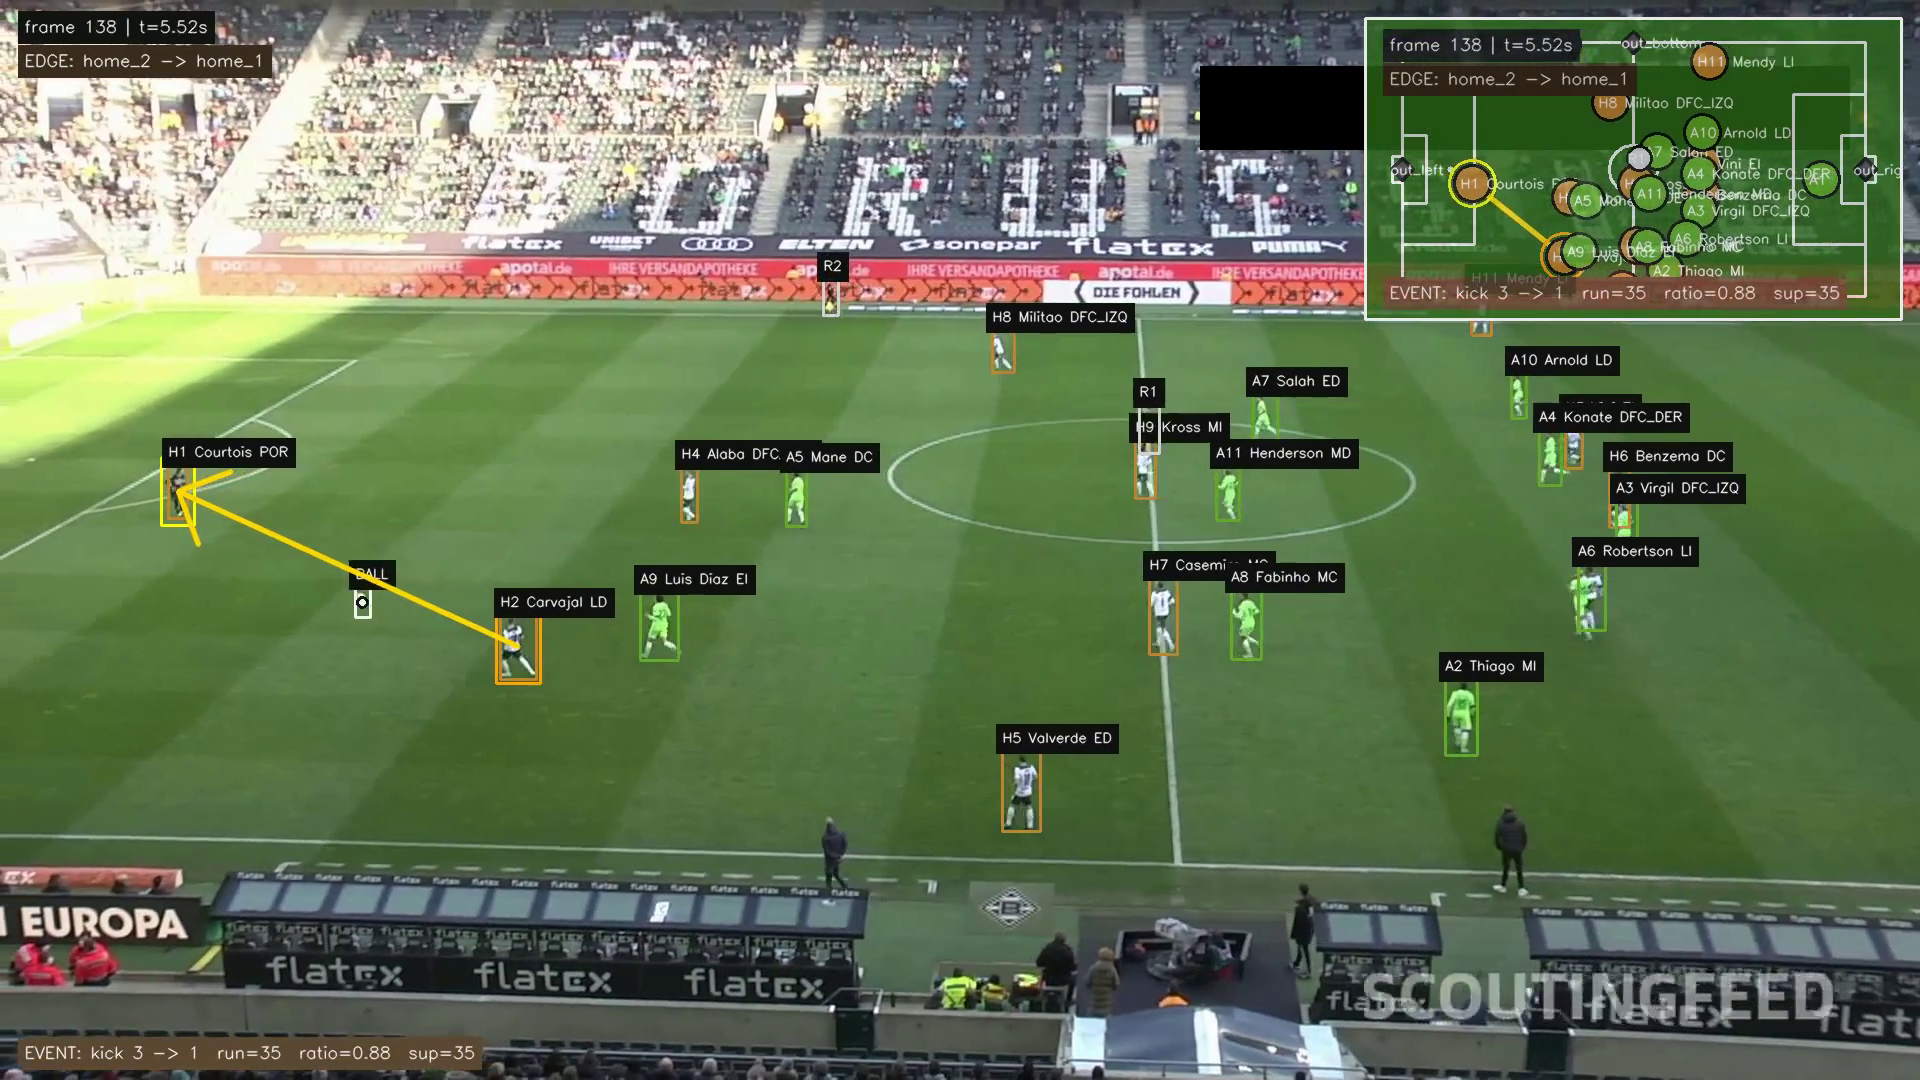
\includegraphics[width=0.95\textwidth]{Imagenes/Propias/tracking_pathcrf_frame.png}
    \caption[Resultado de la clasificación de acciones sobre una ventana temporal]{
    Resultado de la clasificación de acciones sobre una ventana temporal del partido. La salida de PathCRF se consolida mediante postprocesado temporal para obtener un único evento predominante por bloque de emisión, junto con su contexto temporal e identidad de los actores implicados.
    }
    \label{fig:resultado-clasificacion-acciones}
\end{figure}
